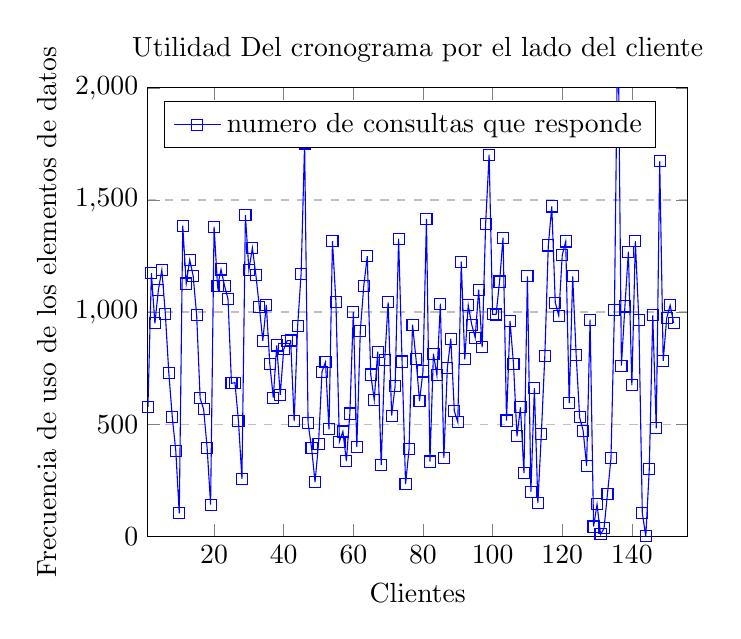
\begin{tikzpicture}
\begin{axis}[
    title={Utilidad Del cronograma por el lado del cliente},
    xlabel={Clientes},
    ylabel={Frecuencia de uso de los elementos de datos},
    xmin=1, xmax=156,
    ymin=0, ymax=2000,
    xtick={},
    ytick={},
    legend pos=north west,
    ymajorgrids=true,
    grid style=dashed,
]

\addplot[
    color=blue,
    mark=square,
    ]
    coordinates {
    %USO EXACTO
    (1,575)
(2,1174)
(3,950)
(4,1098)
(5,1188)
(6,992)
(7,728)
(8,531)
(9,381)
(10,102)
(11,1385)
(12,1127)
(13,1233)
(14,1160)
(15,985)
(16,615)
(17,566)
(18,395)
(19,141)
(20,1381)
(21,1115)
(22,1190)
(23,1117)
(24,1058)
(25,682)
(26,685)
(27,515)
(28,256)
(29,1432)
(30,1187)
(31,1286)
(32,1166)
(33,1024)
(34,872)
(35,1032)
(36,770)
(37,618)
(38,851)
(39,631)
(40,834)
(41,872)
(42,873)
(43,513)
(44,937)
(45,1171)
(46,1752)
(47,505)
(48,393)
(49,242)
(50,411)
(51,734)
(52,777)
(53,477)
(54,1316)
(55,1044)
(56,422)
(57,467)
(58,335)
(59,547)
(60,1001)
(61,397)
(62,916)
(63,1117)
(64,1249)
(65,721)
(66,608)
(67,823)
(68,318)
(69,785)
(70,1043)
(71,538)
(72,670)
(73,1327)
(74,779)
(75,232)
(76,388)
(77,944)
(78,791)
(79,603)
(80,735)
(81,1415)
(82,333)
(83,814)
(84,718)
(85,1037)
(86,349)
(87,751)
(88,881)
(89,559)
(90,509)
(91,1225)
(92,789)
(93,1030)
(94,944)
(95,886)
(96,1100)
(97,843)
(98,1394)
(99,1702)
(100,990)
(101,989)
(102,1136)
(103,1332)
(104,516)
(105,960)
(106,769)
(107,446)
(108,575)
(109,282)
(110,1159)
(111,198)
(112,661)
(113,148)
(114,455)
(115,805)
(116,1297)
(117,1471)
(118,1042)
(119,984)
(120,1254)
(121,1315)
(122,594)
(123,1159)
(124,808)
(125,530)
(126,471)
(127,314)
(128,966)
(129,43)
(130,142)
(131,8)
(132,35)
(133,190)
(134,348)
(135,1009)
(136,2367)
(137,761)
(138,1025)
(139,1269)
(140,673)
(141,1316)
(142,965)
(143,103)
(144,0)
(145,299)
(146,985)
(147,481)
(148,1672)
(149,782)
(150,972)
(151,1030)
(152,951)
    };
    \legend{numero de consultas que responde}

\end{axis}
\end{tikzpicture}

